\documentclass[11pt]{report}
\usepackage[utf8]{inputenc}
\usepackage{bm,amssymb,commath,amsmath}
\usepackage[labelfont=bf]{caption}
\usepackage{graphicx,subcaption,float}
\usepackage[a4paper, total={6in, 8in}]{geometry}
%\usepackage{helvet}

\numberwithin{equation}{section}

%\renewcommand{\familydefault}{\sfdefault}

\graphicspath{ {Figures/} }

\usepackage[backend=biber,style=alphabetic,sorting=ynt]{biblatex}

\addbibresource{bibliography.bib}

\title{Whispering Bloch modes}
%\author{hugo.rakotoarimanga }
\date{\today}

\begin{document}

\maketitle

\tableofcontents

%\chapter{Introduction}

\chapter{Scattering by a single point}

We mainly present in the first three sections the results developed in \cite{evans2007penetration}. We consider a thin elastic plate lying in the $(x,y)$-plane and excited by an incident wave $Re\{\operatorname{u_i}(\bm{r})e^{-i \omega t}\}$, where $\bm{r} = (x,y) = (r cos \theta, r sin \theta)$. The plate undergoes a vertical displacement at temporal frequency $\omega$, normal to its surface, represented by $Re\{\operatorname{u}(\bm{r})e^{-i \omega t}\}$. This displacement obeys to the classical Kirchoff-Love thin-plate theory, and if we introduce the frequency $k$, such that $k^4=m\omega^2/D$ with $D$ known as the bending modulus of the plate and $m$ its surface mass density, under the absence of external forces
%
\begin{equation}
   D(\nabla^4-k^4)\operatorname{u}=0
\end{equation}
%
A fundamental Green function $g$ to the equation,
%
\begin{equation}
    (\nabla^4-k^4)\operatorname{g}(\bm{r},\bm{r'})=\delta(\bm{r}-\bm{r'})
\end{equation}
%
describing a time-harmonic forcing of amplitude $D$ applied to the plate is known to be:
%
\begin{equation}
    \operatorname{g}(\bm{r},\bm{r'}) = C\{\operatorname{H}_0(k\rho)-\operatorname{H}_0(ik\rho)\}    
\end{equation}
%
where $C=i/8k^2$, $\rho=\abs{\bm{r}-\bm{r'}}$ and $\operatorname{H}_0 \equiv \operatorname{H}_0^{(1)}$ is the Hankel function of the first kind and order zero. A derivation of this result using the Hankel transform can be found in \cite{hayek2010}. It is useful for calculations to note that this Green function only depends on the relative distance between points of the $(x,y)$-plane, hence we may adopt a complex representation of points in this plane, thus leading direct calculation on their affixes rather than on their polar or Cartesian coordinates. Another interesting property is that $g$ is bounded as $\rho$ tends to $0$, and as $\rho \rightarrow 0$: 
%
$$\operatorname{g}(\rho) = C + \frac{\rho^2 \ln \rho} {8 \pi} + O(\rho^2)$$
%
$$ \frac{\partial \operatorname{g}}{\partial \rho } \rightarrow 0$$
%
We also have an integral formulation of $\operatorname{g}$, which proves to be useful in order to obtain some results in the next steps
%
\begin{equation} \label{integral}
    \operatorname{g}(\bm{r},\bm{r'}) = \frac{C}{\pi i} \int_{-\infty}^{\infty}  e^{i k (x-x') t} \Big(\frac{e^{-k \lambda(t) \abs{y-y'}}}{\lambda(t)} - \frac{e^{-k \gamma(t) \abs{y-y'}}}{\gamma(t)}\Big) \operatorname{d}t
\end{equation}
%
where
%
\begin{align}
    \lambda(t) &= \begin{cases}
    (t^2-1)^{1/2},& \text{if } \abs{t} \geq 1\\
    i(1-t^2)^{1/2},              & \text{otherwise}
\end{cases}\\
    \gamma(t) &= (1+t^2)^{1/2}
\end{align}
%
We assume that an external point force acts on the origin and that this force is proportional to its displacement by an impedance factor $\mu D$. We can assume that this impedance factor is arises from three different causes: a spring and a damping forces and a concentrated mass, we thus write $\mu D$ as
%
\begin{equation}
    \mu D = M\omega^2 - \kappa - i \omega \nu
\end{equation}
%
where, $\kappa$ and $\nu$ correspond to the spring and damping forces and $M$ is a concentrated point mass. In all the following we consider the case where $\nu = 0$. Using the relation $k^4=m\omega^2/D$, we also introduce non dimensional quantities $\tilde{\mu}$ and $\tilde{\kappa}$ depending only on physical characteristics and not on frequency, introducing a length scale $a$ in the problem
%
\begin{align}
    \tilde{\mu} = \frac{M}{4 m a^2} \quad &\textrm{and} \quad \tilde{\kappa} = \frac{\kappa a^2}{4D}\\
    \mu = 4 k^4 a^2 \tilde{\mu} &- \frac{4 \tilde{\kappa}}{a^2}  
\end{align}
%
The wave can be written with an "amplitude factor" $A$ as
%
\begin{equation} \label{depl}
    \operatorname{u}(\bm{r}) = \operatorname{u_i}(\bm{r}) + A\operatorname{g}(\bm{r},\bm{0})
\end{equation}
%
and we find that $A  = \mu \operatorname{u}(\bm{0})$, where we have set a certain angle of incidence $\psi$ as $\operatorname{u}_i(\textbf{r}) = e^{ikr(\theta-\psi)}$. This last result allows us to express $A$ and $\operatorname{u}(\bm{0})$ in terms of $mu$ and $C$ only:
%
\begin{align*} 
A &= \mu/(1-\mu C) \\ 
\operatorname{u}(\bm{0}) &= 1/(1-\mu C)
\end{align*}
%

\chapter{Scattering by $N$ arbitrary points}

We now extend the previous situation to the case where the incoming wave is scattered by a set of $N$ arbitrary points located at positions $\bm{r_i}$ where $i=1,..,N$, on which a force characterised by an impedance factor $\mu_i D$ acts. We thus generalise  (\ref{depl}) with:
%
\begin{equation}
    \operatorname{u}(\bm{r}) = \operatorname{u_i}(\bm{r}) + \sum_{n=1}^{N} A_n \operatorname{g}(\bm{r},\bm{r_n})
\end{equation}
%
Similarly, we have $A_n = \mu_n \operatorname{u}(\bm{r_n})$ and we obtain a system of equations for the constants $A_n$:
%
\begin{equation} \label{amplitudes}
    \forall m=1,..,N, \ A_m = \mu_m \operatorname{u_i}(\bm{r}) + \mu_m \sum_{n=1}^{N} A_n \operatorname{g}(\bm{r_m},\bm{r_n})
\end{equation}
%
If we let $\mu_m \rightarrow \infty$ (infinite point mass), then we recover the case where the membrane is pinned at the point $\bm{r_m}$ and then (\ref{amplitudes}) becomes
%
\begin{equation}
    \forall n=1,..,N, \operatorname{u}(\bm{r_n}) = A_n / \mu_n   
\end{equation}
%
In that case we have plotted the curve corresponding to the modulus of the plate's displacement at the origin $u_0 = \abs{\operatorname{u}(\bm{0})}$ for two different geometries and angles of incidence. We observe that for a certain normalised frequency $(ka)_{max}$, this displacement is maximal, as shown in the two figures below.
%
\begin{figure} [H]

    \begin{subfigure}{0.5\textwidth}
    \centering
    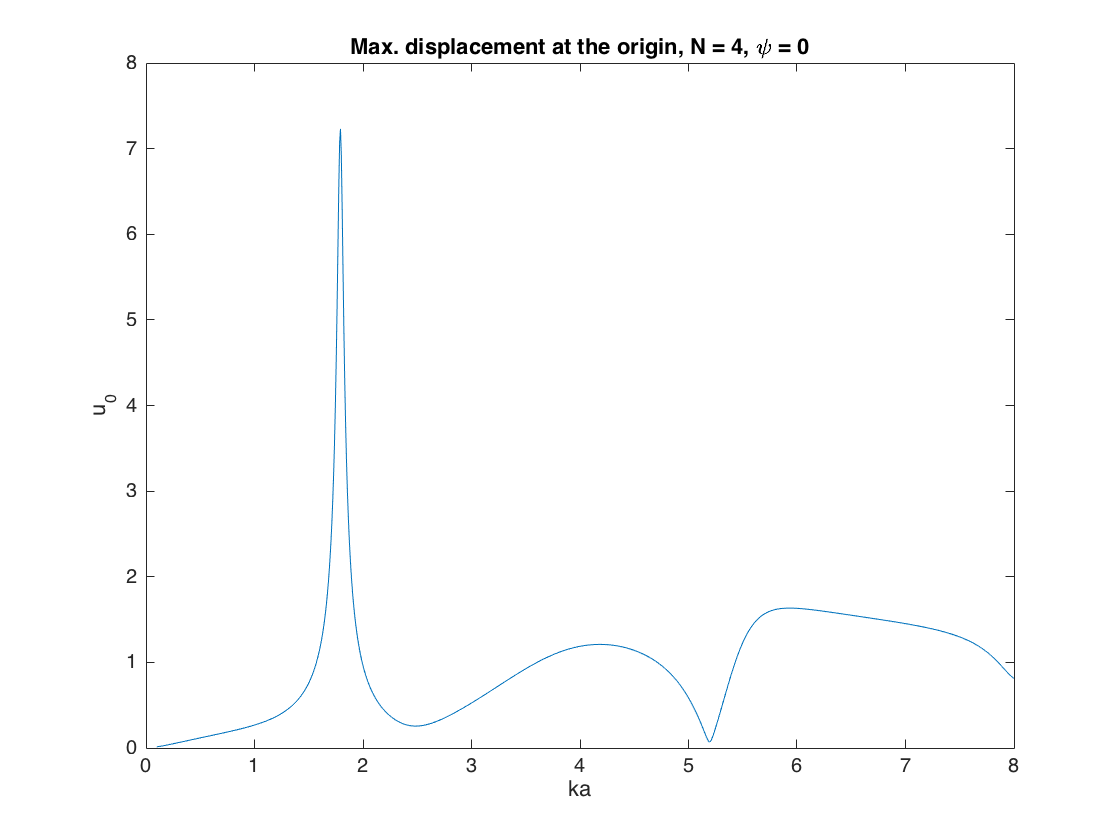
\includegraphics[width = 0.7 \linewidth]{Max_disp4}
    \caption{$N=4$, $\psi = 0$, $(ka)_{max} = 1.792$}
    \label{fig:my_label}
    \end{subfigure}
    \begin{subfigure}{0.5\textwidth}
    \centering
    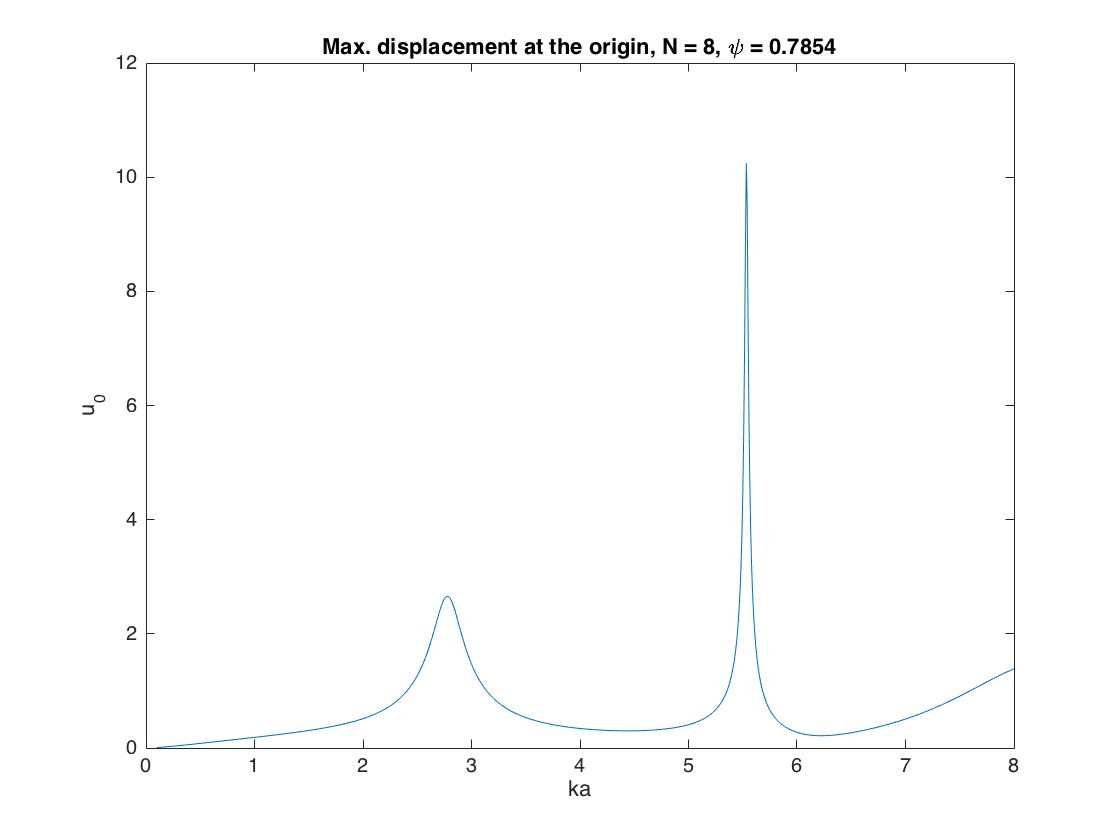
\includegraphics[width = 0.7 \linewidth]{Max_disp8}
    \caption{$N=4$, $\psi = \pi/4$, $(ka)_{max} = 5.532$}
    \label{fig:my_label}
    \end{subfigure}
    
    \caption{Maximum displacement at the origin, pinned points}
\end{figure}

\noindent
The next two figures show the modulus of the wave amplitude for pinned points (i.e. $\mu^{-1} = 0$), for these values of frequency $ka$ and these configurations.
%
\begin{figure}[H]
 
\begin{subfigure}{0.5\textwidth}
\centering
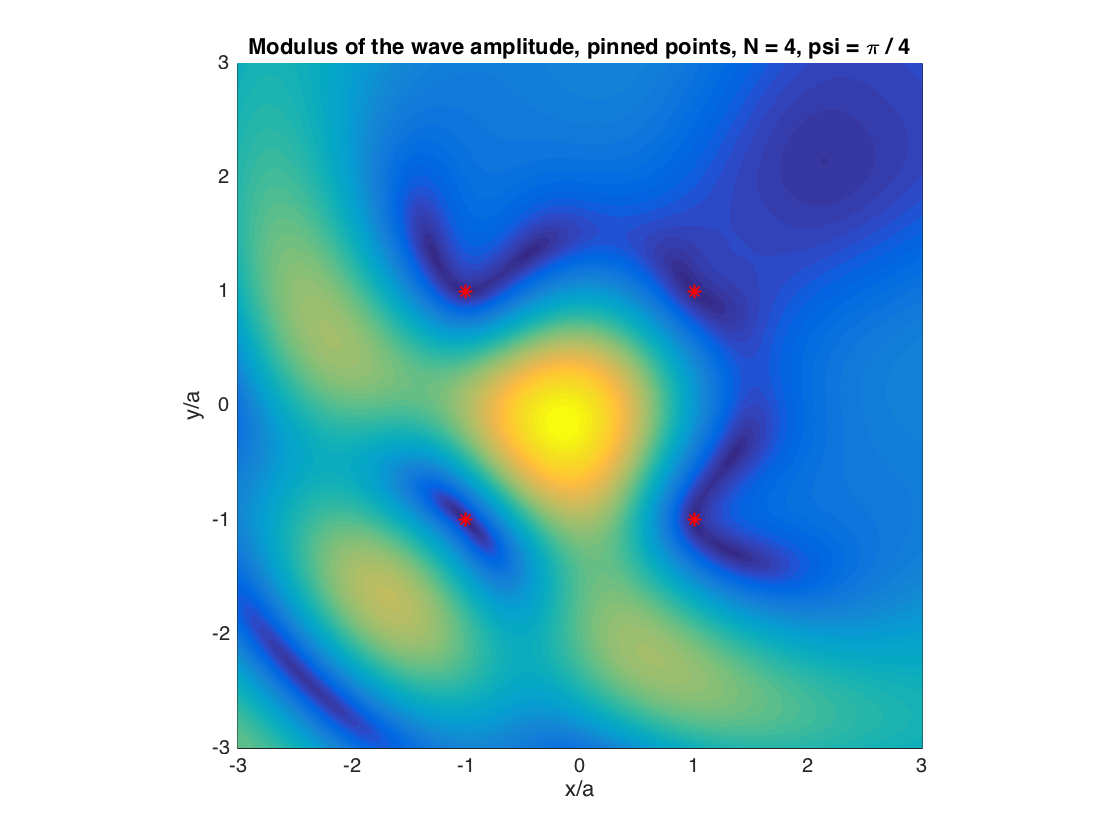
\includegraphics[width=0.8\linewidth]{N4pinned} 
\caption{$ka = 1.792$}
\label{fig:subim1}
\end{subfigure}
\begin{subfigure}{0.5\textwidth}
\centering
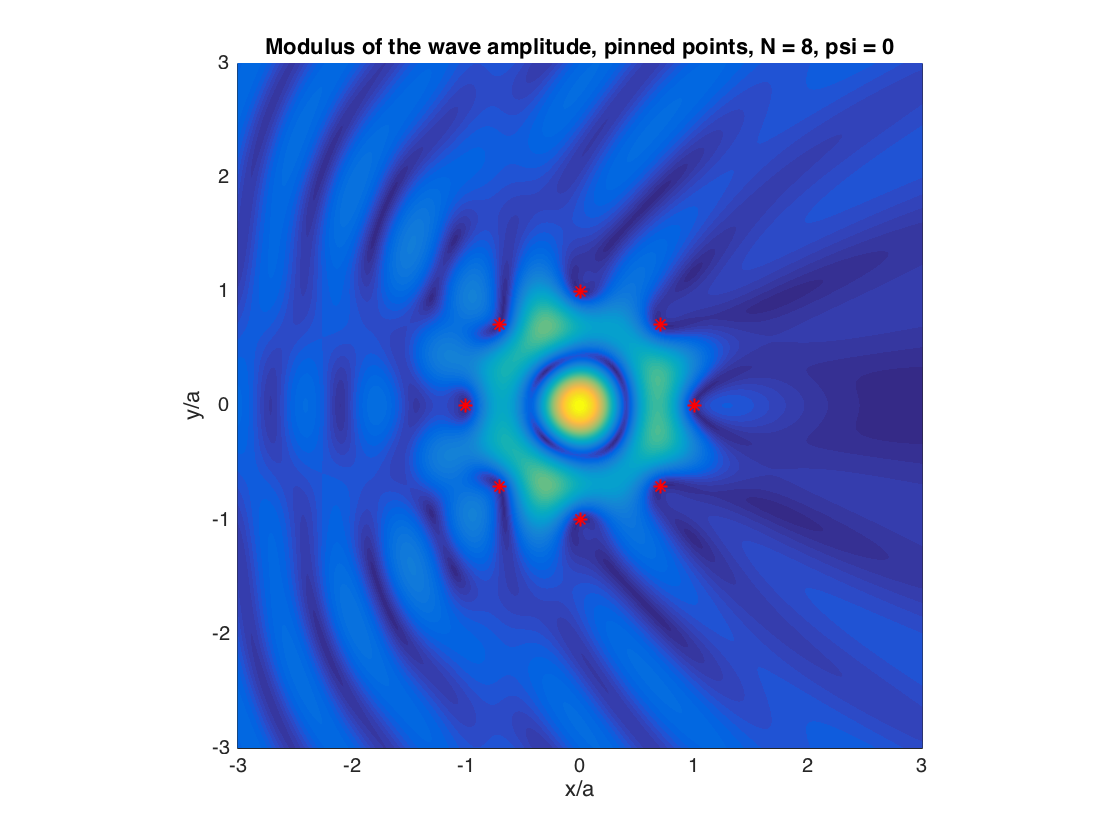
\includegraphics[width=0.8\linewidth]{N8pinned}
\caption{$ka = 5.532$}
\label{fig:subim2}
\end{subfigure}
 
\caption{Modulus of the wave amplitude and scattering by an arbitrary array of pinned points}
\label{fig:image2}
\end{figure}

\chapter{Rayleigh-Bloch modes along an infinite line array of equally spaced points} \label{chap:linear}

In this section, we focus on the existence of Rayleigh-Bloch waves, i.e. localised waves travelling along a periodic array of mass-loaded points. Due to the periodicity $a$ of the array, corresponding to the spacing between the mass-loaded points, we may assume that the amplitude factors at each point are quasi-periodic. We actually apply Bloch's theorem here and in that case, there exist a certain quantity $\beta$ such that
%
\begin{equation}
    \forall n \in \mathbb{Z}, A_n = e^{i\beta a n}A_0
\end{equation}
%
One can show that necessarily $\beta > k$ for this type of wave to exist (\cite{evans2007penetration}). In that case, with the arbitrary amplitude factor $A_0$,
%
\begin{equation} \label{RB}
    u(\bm{r}) = A_0 \sum_{n=-\infty}^{\infty} e^{i\beta a n} \operatorname{g}(\bm{r},\bm{r_n})
\end{equation}
%
We also suppose that each point $\bm{r_n} = (na, 0), n \in \mathbb{Z}$ satisfies the same impedance relation
%
\begin{equation}
    A_n = \mu u(\bm{r_n})
\end{equation}
%
This and  leads to the following dispersion relation
%
\begin{equation} \label{dispersion}
    1 = \mu \operatorname{S}(ka,\beta a)
\end{equation}
%
where
%
\begin{equation}
    \operatorname{S}(ka,\beta a) = \sum_{n=-\infty}^{\infty} e^{i\beta a n} \operatorname{g}(\bm{r},\bm{r_n}) = \frac {1} {4 k^3 a} \sum_{n=-\infty}^{\infty} (\lambda_n^{-1} - \gamma_n^{-1})
\end{equation}
%
This last expression is obtained using the integral representation (\ref{integral}) of the Green's function $\operatorname{g}(\bm{r},\bm{r'})$, Poisson's formula (see \cite{evans2007penetration}), and
%
\begin{align*} 
\lambda_n &= ((\beta_n/k)^2-1)^{1/2} \\ 
\gamma_n &= ((\beta_n/k)^2+1)^{1/2} \\
\beta_n &= \beta + {2 n \pi}/a 
\end{align*}
%
We can solve the dispersion relation (\ref{dispersion}) and obtain the couples $(\beta a, k a)$ such that this relation is satisfied and Rayleigh-Bloch modes exist. The following two figures show the dispersion curves obtained by solving this relation for $\beta a$ and $k a$.

\begin{figure} [H]
    \begin{subfigure}{0.5 \textwidth}
    \centering
    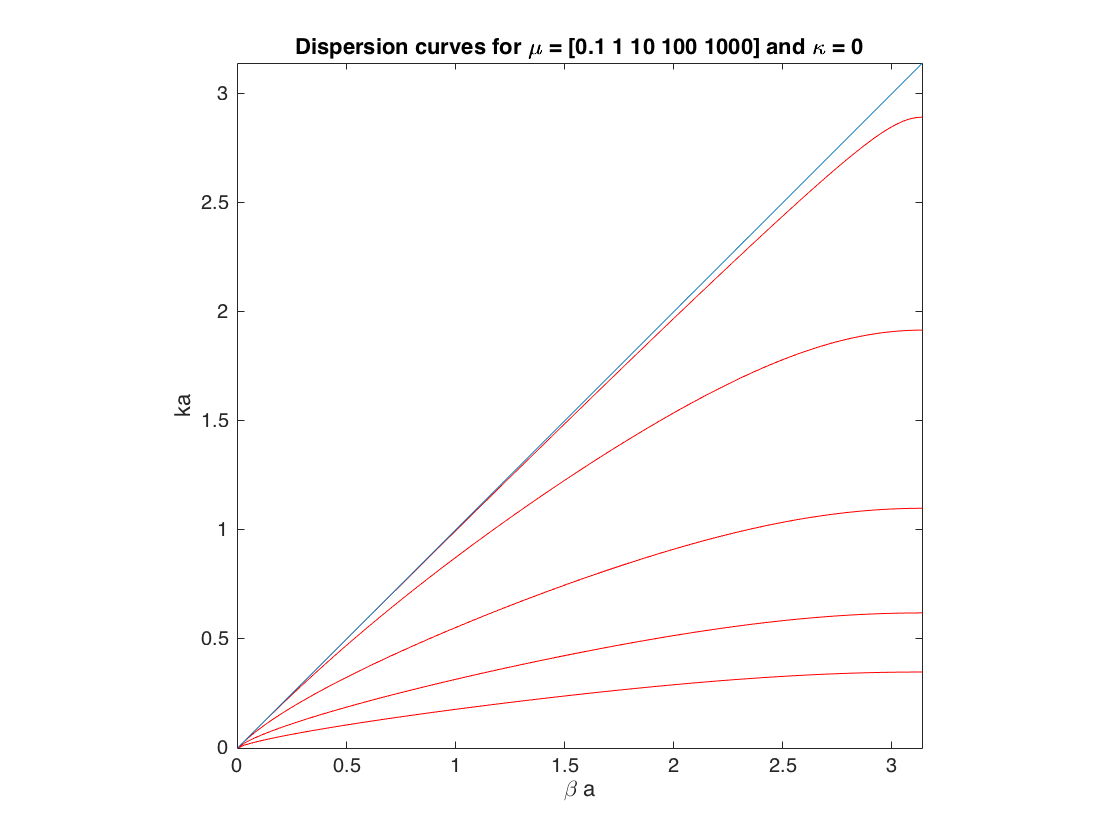
\includegraphics[width = 0.9\textwidth]{Disp_mu}
    \caption{$\tilde{\mu}$ varying and $\tilde{\kappa} = 0$}
    \label{fig:my_label}
    \end{subfigure}
    \begin{subfigure}{0.5 \textwidth}
    \centering
    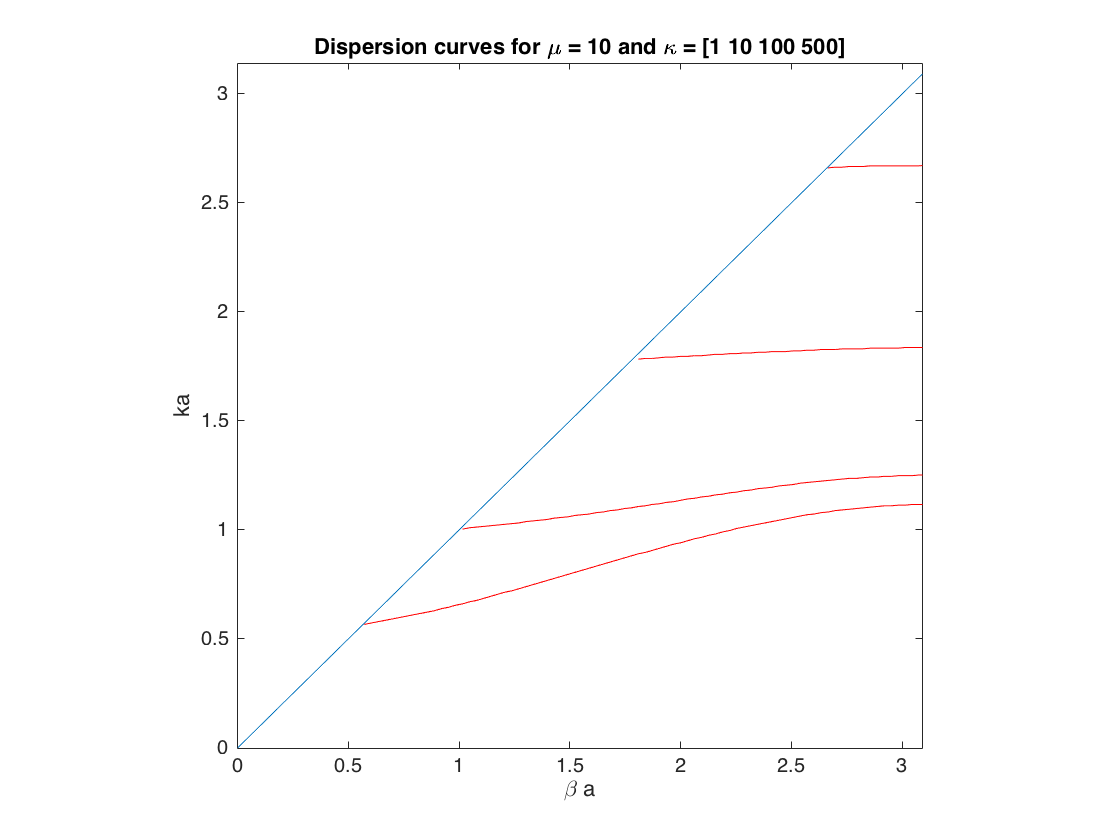
\includegraphics[width = 0.9\textwidth]{Disp_kappa}
    \caption{$\tilde{\kappa}$ varying and $\tilde{\mu}$ fixed ($\tilde{\mu} = 100$)}
    \label{fig:my_label}
    \end{subfigure}
    \caption{Dispersion curves for Rayleigh-Bloch modes along an infinite line of mass-loaded points}
\end{figure}

\chapter{Whispering Bloch modes on a ring of mass-loaded points}

\section{Presentation of the problem}

We now wish to extend the analysis of the existence of the so called whispering Bloch modes, analogous to Rayleigh-Bloch modes on an periodic array of mass-loaded points, to the case of a circular ring of radius $a$ of $N$ equally spaced points. We can derive a version to Bloch's theorem for Bravais lattices in this particular circular geometry. If $A_n, \quad n \in \{0,..,N-1\}$, denotes the amplitude factor at point $n$ then there exist $m \in \{0,.., \lfloor N/2 \rfloor \}$ such that
%
\begin{equation}
    A_n = e^{2 \pi i n m / N}A_0
\end{equation}
%
This gives us a discrete spectrum of whispering Bloch modes when we solve the dispersion relation (\ref{dispersion}). Due to the circular symmetry of this geometry, this relation writes, for a mode $m \in \{0,.., \lfloor N/2 \rfloor \}$
%
\begin{equation}
    1 = \mu(k) \sum_{n=0}^{N-1} e^{2 \pi i n m / N} \operatorname{g}(\bm{r_0}, \bm{r_n};k)
\end{equation}
%
Solving this equation for $k$ gives complex roots and only one of them is of physical significance, i.e. for a give mode indexed by $m \in \{0,.., \lfloor N/2 \rfloor \}$, we only consider frequencies $k$ such that
%
\begin{equation}
    \Re(k) > 0 \quad \textrm{and} \quad \Im(k) < 0
\end{equation}
%
since we are looking for outward going solutions with vanishing energy at infinity. We give below a contour plot of $\log(\abs{\mathcal{D}(k a,m)})$ where
%
\begin{equation} \label{disp_whisp}
\mathcal{D}(k a,m) = \mu(k) \sum_{n=0}^{N-1} e^{2 \pi i n m / N} \operatorname{g}(\bm{r_0}, \bm{r_n};k) - 1
\end{equation}
%
for a fixed $m \in \{0,.., \lfloor N/2 \rfloor \}$.
%
\begin{figure} [H]
    \centering
    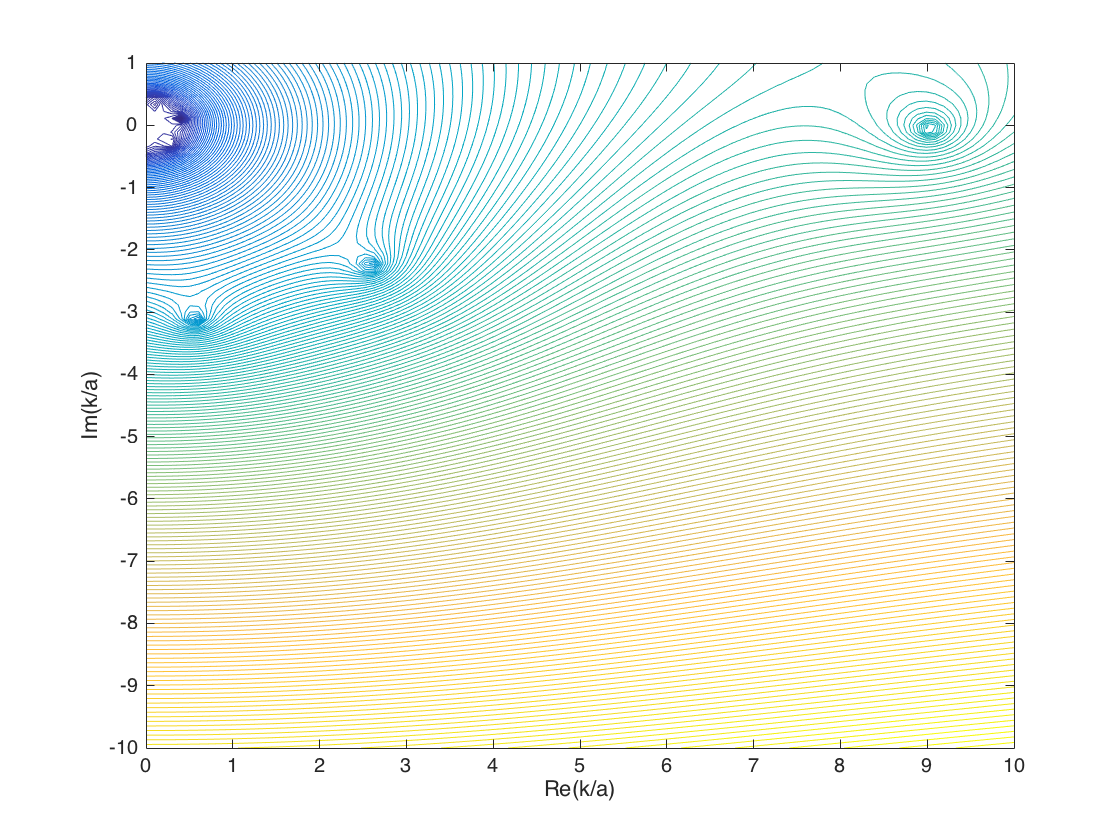
\includegraphics[width = 0.7 \textwidth]{Contour_disp}
    \caption{Contour plot of $\log(\abs{\mathcal{D}(k a,m)})$ for $N =10$, $\tilde{\mu}=1000$ and $m = 5$}
    \label{fig:my_label}
\end{figure}
%
\noindent
In this particular example, $\log(\abs{\mathcal{D}(k a,m)})$ has a minimum located close to the real axis for $k a = 9.03 - 0.05i$. This corresponds to a zero of the dispersion relation $\mathcal{D}(k a,m)$. We seek for solutions near the real axis as we are looking for confined modes. Otherwise, the other modes have too much leaking energy. For this value, we plot the corresponding real part of the wave amplitude $\operatorname{u}(\bm{r})$ below.
%
\begin{figure} [H]
    \centering
    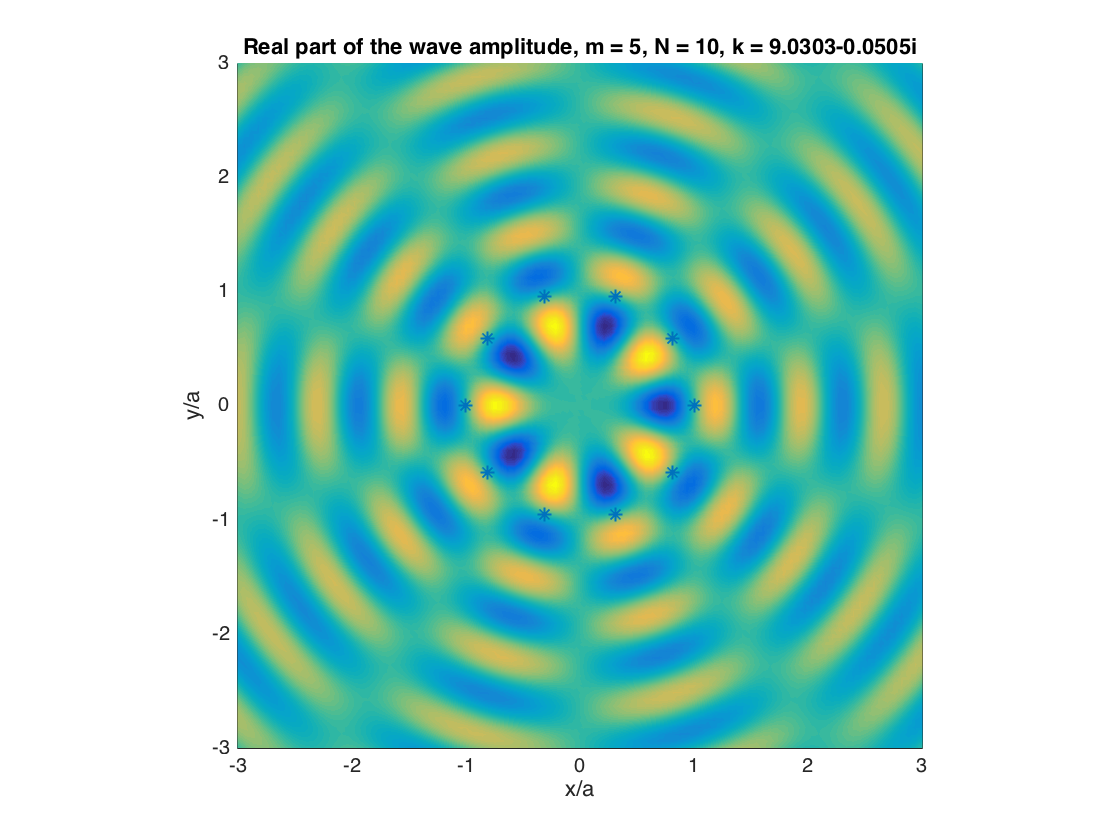
\includegraphics[width = 0.7\textwidth]{RB10_5}
    \caption{Whispering Bloch mode ($m=5$) on a ring $N=10$, $k a = 9.03 - 0.05i$ }
    \label{fig:my_label}
\end{figure}
%
\noindent
A first remark can be made on the numerical solving of the dispersion  relation for a fixed $m$. When calculating the values of $\mathcal{D}(k a,m)$, one can notice that these values are very high except for the very thin peaks where $\mathcal{D}(k a,m)=0$. Calculating $\log(\abs{\mathcal{D}(k a,m)})$ and trying to find its minima is not very helpful since it does not eliminate the problem of the peaks' thinness, and lacks automation. We now want to further analyse the whispering Bloch modes for this ring geometry. In particular, as in section \ref{sec:linear}, we need to plot the discrete dispersion curves for the whispering Bloch modes corresponding to this geometry. For this, we can use the method suggested by \cite{delves1967numerical} and \cite{brazier1991} in order to find the complex zeros of the dispersion relation $\mathcal{D}(k a,m)$ located near the real axis in the lower right quadrant $\{z \in \mathbb{C}, \quad \Re(z)>0, \quad \Im(z)<0 \}$. Other interesting figures to obtain could be the influence of the non-dimensional mass-loading factor $\tilde{\mu}$ and of the number of mass-loaded points $N$ on some quantity $Q$ analogous to a factor of quality, characterising energy confinement in the structure.

\section{An algorithm for complex root finding}
We present here the idea exposed in \cite{delves1967numerical} and \cite{brazier1991} to implement an algorithm capable of finding the complex roots of a certain function $f(z)$, e.g. a dispersion relation. This is equivalent to finding the poles of $F(z) = 1/f(z)$. First of all, the argument principle provides us with an elegant way of counting the numbers of zeros and poles of $F$ in a given region of the complex plane.\\

\paragraph{The winding number as an indicator of the presence of poles}
We introduce the winding number of the function $F(z) = 1/f(z)$ assumed to be analytic over a region of the complex plane, enclosed by the counterclockwise contour $\mathcal{C}$ containing $n_p$ simple poles and, for more generality $n_z$ zeros, as
%
\begin{equation} \label{winding}
    w = \frac{1}{2 \pi i}\oint_{\mathcal{C}} \frac{F'(z)}{F(z)} \operatorname{d}z = n_z - n_p
\end{equation}
%
Note that (\ref{winding}) is an analytical continuation of $\log F$ on the contour $\mathcal{C}$.\\

Hence, in order to calculate the winding number (\ref{winding}) we do not need to actually compute the derivative $F'(z)$ but only to count the number of times $\log F$ crosses the negative real axis $\{ z \in \mathbb{C}, \quad \operatorname{arg}(z) = - \pi \}$, where the branch cut of $\log F$ occurs. We increment this number when it crosses from above and decrease it when $\log F$ crosses from below. It can be difficult to implement in an algorithm and this difficulty arises from discretisation. \cite{delves1967numerical} proposes some ideas to solve the difficulties of the numerical implementation of this algorithm.\\

The logarithm has a branch cut for $z$ such that $\operatorname{arg}(z) = - \pi$. Thus, we need to keep track of the points where $\operatorname{arg}\{F(z)\} = - \pi$.  We set $\mathcal{C}$ to be the circle $\{ z \in \mathbb{C}, \quad \abs{z} = r > 0 \}$. To avoid confusion, for $z = r e^{2 \pi i t} \in \mathcal{C}$, we only refer here to the principal value of $\log F$, i.e.
%
\begin{equation}
    \log F(z) = \log F(r e^{2 \pi i t}) \quad \textrm{} \quad -1/2 < t \leq 1/2
\end{equation}
%
The mapping $z \mapsto w = F(z)$ maps the circle $\mathcal{C}$ on a closed curve $\mathcal{\tilde{C}}$ in the complex $w$-plane. Assume that this curve crosses the negative real axis in the $w$-plane at $m$ points $q_1, q_2, ..., q_m$, such that
%
\begin{equation}
    q_j = F(p_j) \quad \textrm{with} \quad \operatorname{arg}(q_j) = - \pi
\end{equation}
%
In theory to each $q_j$ we would attribute a number $\sigma_j$ equal to $+1$ or $-1$ according to the direction in which $\mathcal{\tilde{C}}$ crosses the negative real axis ($+1$ if counter-clockwise), and the sum of these would give the winding number. For $j \in \{1,...,m\}$, $p_j \in \mathcal{C}$ in the $z$-plane, and we write
%
\begin{equation}
    p_j = r e^{2 \pi i T_j}
\end{equation}
%
Assume that the circle $\mathcal{C}$ is discretised in $P$ points, $r e^{2 \pi i t_j}$ and that the argument as calculated by the computer lies between $-\pi$ and $\pi$. We dispose of the discretised values of the function $F_j = F(r e^{2 \pi i t_j}) \in \mathcal{\tilde{C}}$. Then to each $t_j$ we can associate a number $s_j$ such that
%
\begin{align*}
    s_j = + 1 \quad &\textrm{if} \quad \operatorname{arg}(F_j) -   \operatorname{arg}(F_{j-1}) \leq -\pi\\
    s_j = 0 \quad &\textrm{if} \quad  -\pi < \operatorname{arg}(F_j) -   \operatorname{arg}(F_{j-1}) \leq \pi\\
    s_j = - 1 \quad &\textrm{if} \quad \pi < \operatorname{arg}(F_j) -   \operatorname{arg}(F_{j-1})
\end{align*}
%
with $T_{-1} = T_P$. Hence if $T_k$ lies between $t_k$ and $t_{k+1}$ we have $s_{k+1} = \sigma_k$ thanks to the mapping $w = F(z)$. Thus 
%
\begin{align*}
    \operatorname{card}(\{j \in \{1,..,P\}, \quad s_j = +1\})&=\operatorname{card}(\{k \in \{1,..,m\}, \quad \sigma_k = +1\}) \\
    \operatorname{card}(\{j \in \{1,..,P\}, \quad s_j = -1\})&=\operatorname{card}(\{k \in \{1,..,m\}, \quad \sigma_k = -1\})
\end{align*}
%
and the value of the sum of the $(s_j)$ and of the $(\sigma_k)$ is the same
%
\begin{equation}
    \sum_{j=1}^P s_j = \sum_{k=1}^m \sigma_k =  n_z - n_p =\frac{1}{2 \pi i}\oint_{\mathcal{C}} \frac{F'(z)}{F(z)} \operatorname{d}z
\end{equation}
%
\paragraph{Moments of the winding number}
The previous method allows us to conveniently calculate the winding number of $F$ in any circular region, with the appropriate translation of the circle $\mathcal{C}$. This number allows us to know if zeros or poles are contained in the region enclosed by $\mathcal{C}$, assuming that no zeros or poles lie on the contour $\mathcal{C}$ itself. However, using a corollary of the argument principle, we can even obtain the location of these in the complex plane. This corollary gives a relation between $n$-th moment of $F'/F$ and the positions of the zeros $z_{z,i}$ and poles $z_{p,i}$ of $F$,
%
\begin{equation} \label{moments}
    I_n =     \frac{1}{2 \pi i}\oint_{\mathcal{C}} z^n \frac{F'(z)}{F(z)} \operatorname{d}z = \sum_i z_{n,i}^{n} - \sum_i z_{p,i}^{n} 
\end{equation}
%
A convenient way to evaluate (\ref{moments}) computationally is by using an analytical continuation of $\log F$ on $\mathcal{C}$ and performing an integration by parts
%
\begin{equation} {\label{IPP}}
     I_n = \frac{1}{2 \pi i} \Big( [z^n \log F(z) ]  - n \oint_\mathcal{C} z^{n-1} \log F(z) \operatorname{d}z \Big)
\end{equation}
%
If we divide the contour $\mathcal{C}$ accordingly to the discontinuities of $\log F(z)$ occurring at $p_1,..., p_m$, then (\ref{IPP}) becomes
%
\begin{equation}
    I_n = \frac{1}{2 \pi i} \Big( \sum_{j=1}^m z^n \log F(z) \Bigr|_{{\substack{p_j^{+}\\p_{j+1}^{-}}}}  - n \oint_\mathcal{C} z^{n-1} \log F(z) \operatorname{d}z \Big)
\end{equation}
%
or
%
\begin{equation}
    I_n = \frac{1}{2 \pi i} \Big( \sum_{j=1}^m \sigma_j p_j^n  - n \oint_\mathcal{C} z^{n-1} \log F(z) \operatorname{d}z \Big)
\end{equation}
%
In particular,
%
\begin{equation}
    I_1 = \frac{1}{2 \pi i} \Big( \sum_{j=1}^m 2 \pi i \sigma_j p_j  -  \oint_\mathcal{C} \log F(z) \operatorname{d}z \Big) = \sum_i z_{n,i} - \sum_i z_{p,i}
\end{equation}
%
and the second integral in this expression is
%
\begin{equation}
	\oint_\mathcal{C} \log F(z) \operatorname{d}z = 
	\int_0^{2\pi} i r e^{i\theta} \log F(r e^{2\pi i\theta}) \operatorname{d}\theta
\end{equation}
%
which we can approximate by
%
\begin{equation}
	\oint_\mathcal{C} \log F(z) \operatorname{d}z \simeq \frac{2 \pi i}{P} \sum_{j=1}^{P} re^{2 \pi i t_j} F(r e^{2 \pi i t_j})
\end{equation}
%
and then
%
\begin{equation}
	I_1 = \sum_i z_{n,i} - \sum_i z_{p,i} \simeq  \sum_{j=1}^m \sigma_j p_j  - \frac{1}{P} \sum_{j=1}^{P} re^{2 \pi i t_j} F(r e^{2 \pi i t_j}) 
\end{equation}
%
One can notice, that these results still hold by performing a translation of the contour $\mathcal{C}$ so that we consider the circle of center $c$ and radius $r$.\\
\noindent
Returning to the case where we know that $f$ only has zeros, i.e. $F$ only has poles ($n_z = 0$), we can combine these ideas to form the following simple algorithm
%
\begin{enumerate}
    \item Construct a counterclockwise contour $\mathcal{C}$, typically a circle of center $c$ and radius $r$ small enough
    \item Define a region of the complex plane to scan for poles
    \item Move  $\mathcal{C}$ in this region and evaluate the winding number for each position:
        \begin{enumerate}
        \item if the winding number is -1 then
            \begin{equation*}
                I_1 =  - z_p
            \end{equation*}
        \end{enumerate}
    \item Move to the next position.
\end{enumerate}
%
\paragraph{A variation}
One may remark that using the different moments of the winding number, it is possible to calculate the positions of the zeros and poles when the contour $\mathcal{C}$ encloses more than one pole or zero of $F$. Let $\mathcal{C}$ be a fixed contour, in the general case where $F$ has both zeros and poles lying in $\mathcal{C}$, recall (\ref{moments}), giving the $n$-th moment of the winding number as
%
\begin{equation}
  I_n = \sum_i z_{n,i}^{n} - \sum_i z_{p,i}^{n}
\end{equation}
%
The winding number gives us an indication of the numbers of poles and zeros lying in the region enclosed by $\mathcal{C}$. Let us return to the case where we know that $F(z) = 1/f(z)$ has only poles. Suppose that in the previous algorithm we designed, the radius of the contour we use for exploring a specific part of the complex plane is too big so that it ignores a region for which the winding number is strictly below $-1$. This means that the region delimited by $\mathcal{C}$ contains more than two poles, $z_{p,1}$, ..., $z_{p,k}$, $k \geq 2$. In that configuration, denoting $-I_n$ by $J_n$ for convenience
%
\begin{equation}
  \sum_{i=1}^k z_{p,i}^{n} = -I_n = J_n
\end{equation}
%
For $n,k \geq 1$, we recall here the elementary symmetric polynomials $e_1(X_1,\ldots,X_k),\ldots,\\ e_n(X_1,\ldots,X_k)$ so that
%
\begin{equation}
  e_m(X_1,...,X_k) = \sum_{1\leq j_1 < j_2 <...<j_k\leq k} X_{j_1}\ldots X_{j_k}
\end{equation}
%
and $e_n(X_1,...,X_k) = 0$ if $n > k$. Then using the fact that a polynomial $Q$ with roots $z_{p,1},\ldots,z_{p,k}$ can be written of the elementary symmetric polynomial as
%
\begin{equation}
	Q(z) = \prod_{i=1}^k \left(z-z_{p,i}\right) = \sum_{j=0}^k \left(-1\right)^{k+j}e_{k-j}\left(z_{p,1},\ldots, z_{p,k}\right)z^j
\end{equation}
%
Finally, recalling Newton's identities, for $j \in \left\{1,..,n\right\}$
%
\begin{equation}
	e_{j}\left(z_{p,1},.., z_{p,k}\right) = \frac{1}{j}\sum_{i=1}^j (-1)^{i-1} e_{j - i} \left(z_{p,1},\ldots, z_{p,k}\right) J_i
\end{equation}
%
Since $e_0 = 1$ this gives a nice recurrence formula for calculating the coefficients of the polynomial $Q$. Thus the problem of finding the poles of $F$ in a certain region breaks done to the computation of the roots of $Q$, provided we know the number of poles in that region and that we have approximated the moments $I_n$ following the method we described in the previous paragraph.

\paragraph{An example when $w=-2$} Obviously, for a larger $k$ if $w = -k$, signifying the contour encloses $k$ poles of $F$, the research of poles comes at a heavier computational cost. However, when $k=2$ the variation detailed above can prove to be useful, since it allows for more flexibility when choosing the contour $\mathcal{C}$ and especially its radius. A circle with a larger radius enables a faster "scanning" of the region and decreases the risk of missing out some poles. In that case, the relations written above have a nicer formulation. We write
%
\begin{align}
	e_0 = e_0(z_{p,1},z_{p,2}) &= 1\\
	e_1 = e_1(z_{p,1},z_{p,2}) &= J_1(z_{p,1},z_{p,2})\\
	e_2 = e_2(z_{p,1},z_{p,2}) &= \frac{1}{2}\left(J_1(z_{p,1},z_{p,2})^2 - J_2(z_{p,1},z_{p,2})\right)
\end{align}
%
where
%
\begin{align}
	J_1(z_{p,1},z_{p,2}) &= -(z_{p,1}+z_{p,2}) = -I_1 \\
	J_2(z_{p,1},z_{p,2}) &= -(z_{p,1}^2+z_{p,2}^2) = -I_2	
\end{align}
%
Therefore, the two poles of $F$ lying inside $\mathcal{C}$,  $z_{p,1}$ and $z_{p,2}$ are the roots of the polynomial
%
\begin{equation}
	Q(z) = e_2 - e_1 z + e_0 z^2 
\end{equation}
%
i.e.
%
\begin{equation}
	Q(z) = \frac{1}{2}(I_1^2 + I_2) + I_1 z + z^2
\end{equation}
%

\section{Application the the analysis of the whispering Bloch modes}

\paragraph{Quality factor}
In the previous section we have given the details of an algorithm for finding the complex roots of a function. We apply this to the relation dispersion $\mathcal{D}(k,m)$ (\ref{disp_whisp}) to produce graphs showing the influence of the different geometrical and physical parameters such as the number of mass-loaded points $N$, the mass-loading parameter $\tilde \mu$, on the confinement of the modes inside the ring stucture. To do so, we introduce the non dimensional quality factor $Q$ as follows,
%
\begin{equation}
	Q = \frac{\Re\left\{k^2\right\}}{2\abs{\Im\left\{k^2\right\}}}
\end{equation}
%
as a measure of this confinement. The higher $Q$ is, the better the energy is confined in the ring and does not leak out.

\paragraph{Influence of $N$} For $N = 2,4,\ldots,30$, focusing our analysis on the symmetrical mode corresponding to $m=N/2$, we have solve for $k$ in the relation dispersion and calculated the corresponding quality factors. This gave us the following graph, showing the influence of the number of points.

\begin{figure} [H]
    \centering
    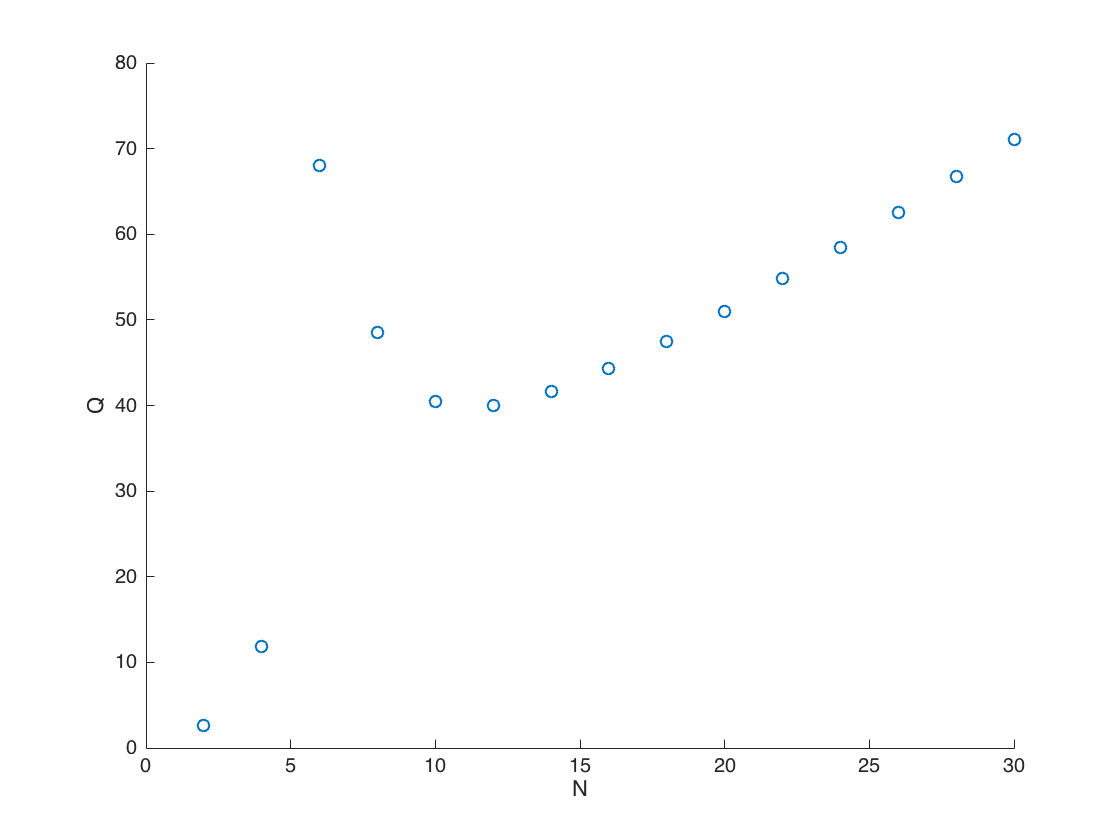
\includegraphics[width = 0.5\textwidth]{Influence_of_N}
    \caption{Influence of $N$ for $m=N/2$ on $Q$, $\tilde \mu = 1000$}
    \label{fig:my_label}
\end{figure}

\noindent
We notice that the $Q$ factor has a local maximum for $N=6$ and a local minimum at $N=10$. As we may expect, the efficiency of the energy confinement grows as the number of points on the ring increases.

\paragraph{Influence of $\tilde \mu$} We are now interested in the influence of the mass-loading parameter.

\begin{figure} [H]
    \centering
    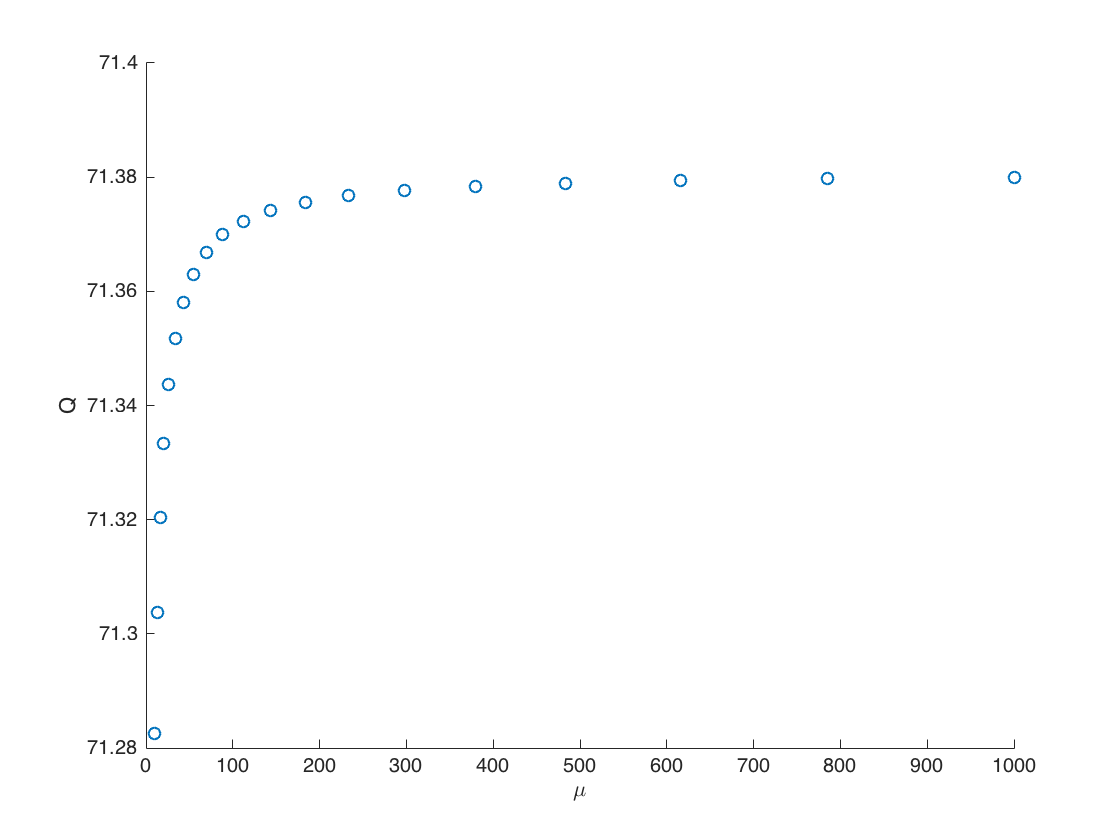
\includegraphics[width = 0.7\textwidth]{Influence_of_mu}
    \caption{Influence of $\tilde \mu$ for $N=30$, $m=15$}
    \label{fig:my_label}
\end{figure}

\noindent
We observe a saturation phenomenon. For $\tilde \mu$ greater than approximately $500$ the mass-loading has no further influence on the quality factor $Q$. We also note that the variations of $Q$ induced by the mass-loading are small.% We can observe the cumulated effects of the changes of $N$ and $\tilde \mu$ on the quality factor in the next figure.

\paragraph{Dispersion plots} For $N=30$ we give below the dispersion curve corresponding to the values of $k$ plotted against the Bloch mode $m$. As expected, those curves are symmetrical with respect to $m=N/2$.

\begin{figure} [H]
    \centering
    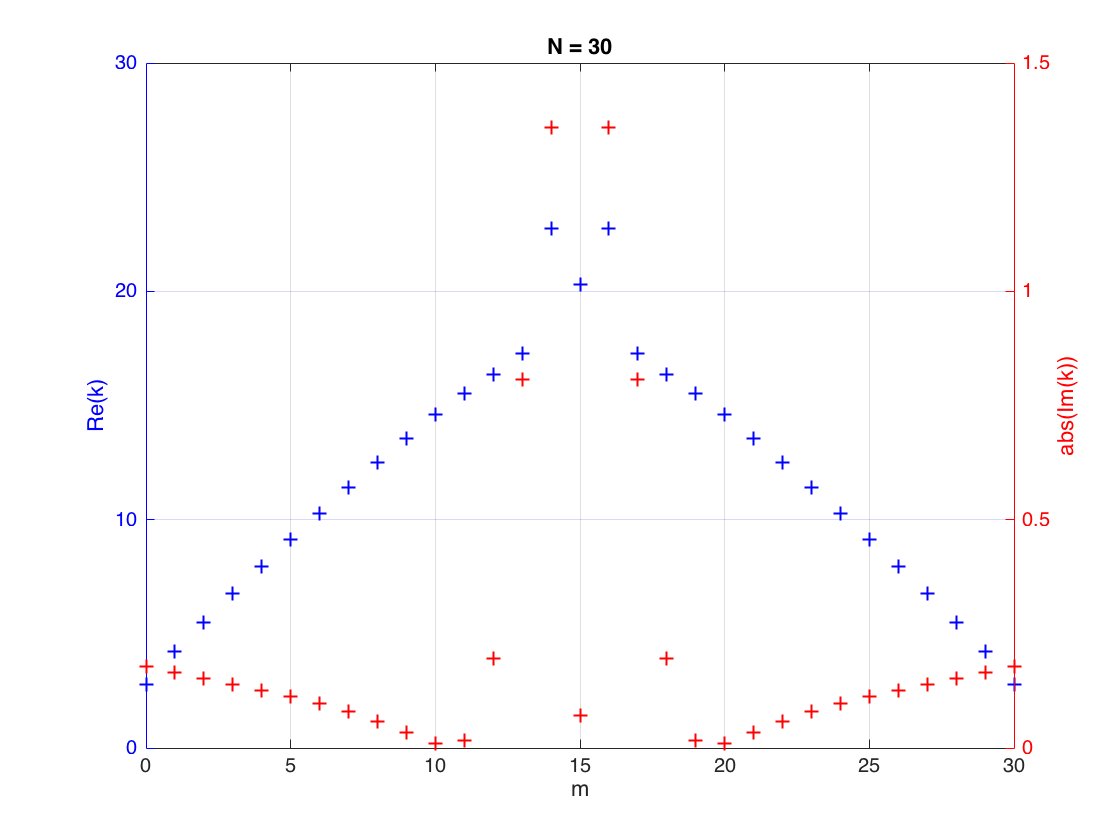
\includegraphics[width = 0.7\textwidth]{m_symmetric}
    \caption{Dispersion curves for $N=30$, $\tilde \mu = 1000$}
    \label{fig:my_label}
\end{figure}

\listoffigures

\newpage

\printbibliography

\end{document}
